\section{Дискретный пример}
Рассмотрим ту же самую модель электродвигателя, что и в позапрошлой секции. Но теперь будем предполагать, что управление запаздывает на $h = 0,\!05$, а периодичность наблюдений $\varepsilon = 0,\!2$.

Проведем редукцию той системы к дискретной. Посчитаем все матрицы численными методами.
$$
x^{k+1} = \Phi x^k + \Gamma_1 u^k + \Gamma_2 u^{k-1},
$$
где
$$
        \Phi = e^{A\varepsilon} \approx \begin{pmatrix}
\;\;\,0,\!6705 & -0,\!0013 \\
-0,\!0669 & \;\;\,0,\!1354
        \end{pmatrix},
$$
$$
        \Gamma_1 = \int\limits_{h}^{\varepsilon}
        e^{As}\,ds \cdot B \approx
\begin{pmatrix}
\;\;\,0,\!2345 \\
-0,\!0175
\end{pmatrix}, 
$$
$$
        \Gamma_2 = \int\limits_{0}^{h}
        e^{As}\,ds \cdot B \approx
        \begin{pmatrix}
\;\;\,0,\!0952 \\
-0,\!0021
        \end{pmatrix}.
$$
Убедиться в том, что построенная система действительно приближает исходную можно на рисунке Рис.~\ref{img:cont-and-disc}.
\begin{figure}[bh]
        \noindent\centering{
        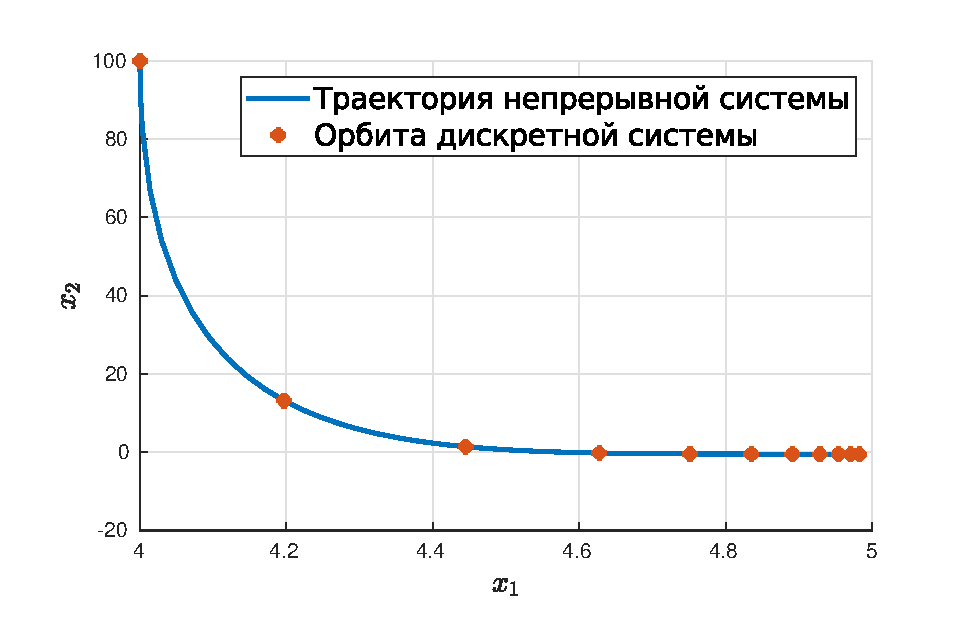
\includegraphics[width=160mm]{content/discrete-example/cont-and-disc.eps}
        }
        \caption{Траектория непрерывной системы и орбита соответствующей редуцированной дискретной системы выпущенной из начальной точки $x_0 = [4,\, 100]\T$ с постоянным управлением $u \equiv 1$.}
        \label{img:cont-and-disc}
\end{figure}

Оставим все абсолютно так же и посмотрим на графики координат и оптимального управления.
\begin{figure}[bh]
        \noindent\centering{
        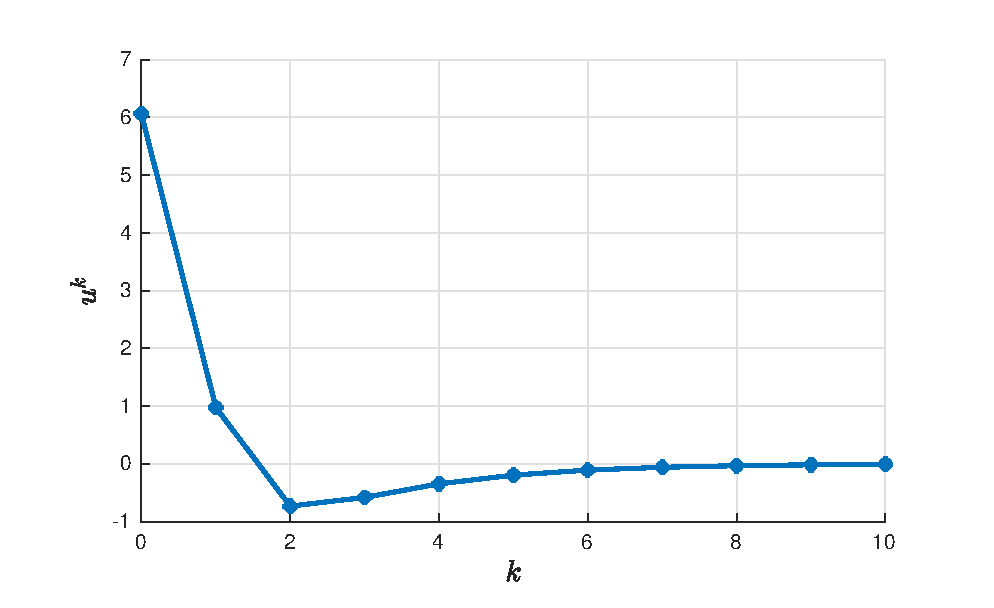
\includegraphics[width=160mm]{content/discrete-example/discr_control.eps}
        }
        \caption{.}
        \label{img:discr_control}
\end{figure}
\begin{figure}[bh]
        \noindent\centering{
        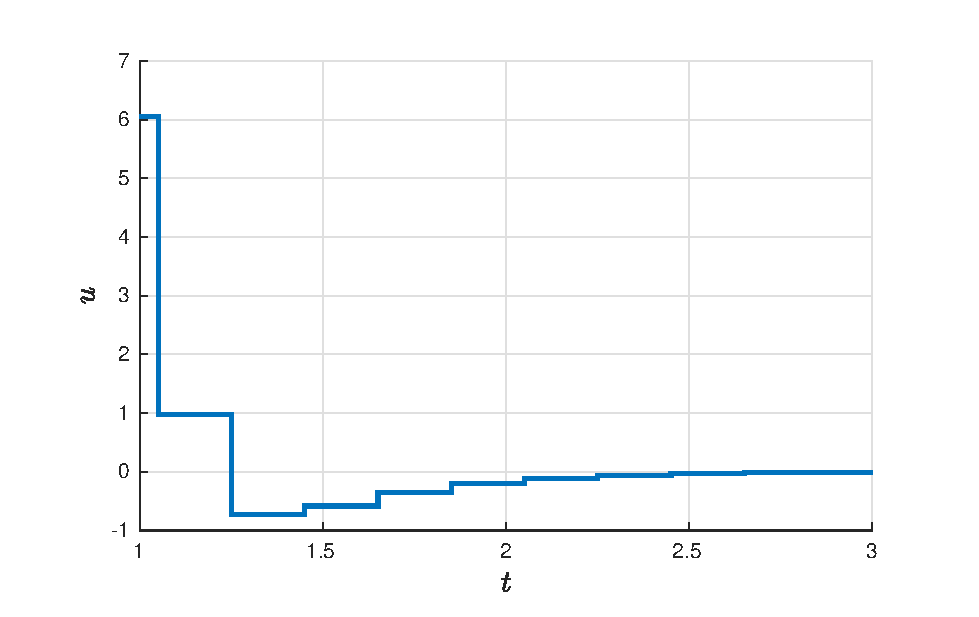
\includegraphics[width=160mm]{content/discrete-example/control.eps}
        }
        \caption{.}
        \label{img:control}
\end{figure}
\begin{figure}[bh]
        \noindent\centering{
        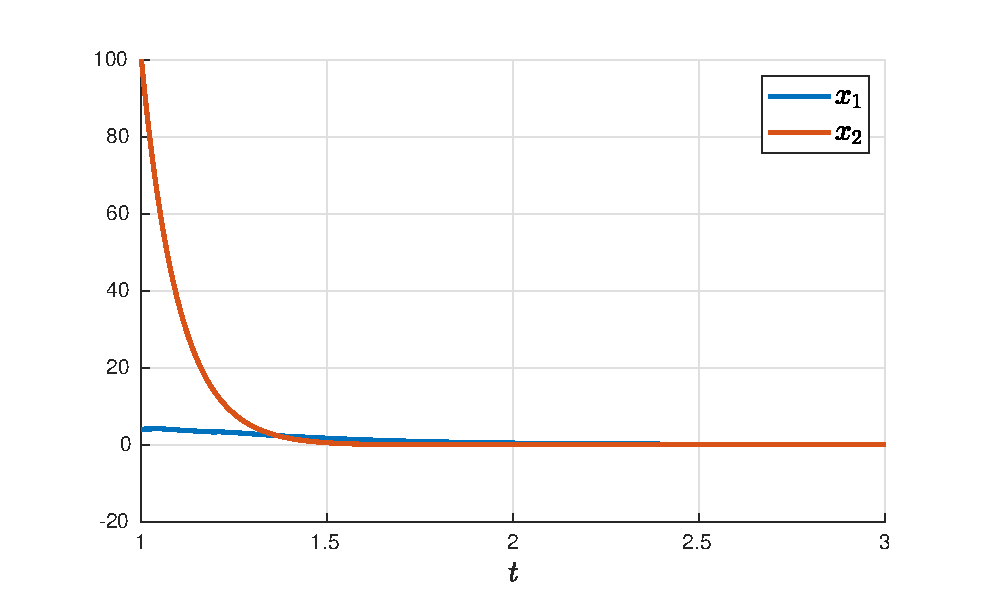
\includegraphics[width=160mm]{content/discrete-example/coords.eps}
        }
        \caption{.}
        \label{img:coords}
\end{figure}
